\part{Analysis}
In this section, we will attempt to give the reader insight into the rationale behind the decisions made in this project, by reflecting on challenges uncovered by analysing the problem area. 

The section is structured by the various techniques and artefacts used in conducting the analysis. The primary topics covered in this section are:
\begin{itemize}
\item Business modelling
\item Requirements analysis
\item Data modelling
\item Architectural analysis
\end{itemize}
We begin the section by investigating and discussing the business model on which the requirements of system are based.

\section{Business modelling} \label{BusinessModel}
The following will present a business model which will demonstrate the main ideas, advantages, and possible threats behind our system.

Throughout the extreme growth of the usage of the Internet, a similar growth has been seen for user-uploaded content, which have exploded on sites like Youtube and Facebook. Especially media files, like video, pictures, and music have surfaced all over these sites, mainly due to the emergence of smartphones with picture and video capturing capabilities, and the democratization of media editing software !!REFERENCE TIL LAWRENCE LESSIG TED TALK. Our business concept takes advantage of these trends, by letting users share video tutorials with the RentIt service.

Tutorials have been widely exposed on the Internet, where people are using them to find solutions on how to do things themselves. Because of this, we have decided to develop a system where a user can download and upload home made tutorials and get paid for providing these files for the system. We expect that getting payment for creating tutorials will encourage authors to create videos of a very high quality. The payments will be financed by users buying or renting tutorials.

\subsection{Target Group}
The target group is expected to posses general IT knowledge and know how to use a computer at a basic level. More specifically, the system will target users who have a specific issue they need a solution for, and also users that want to learn and their expand their knowledge of a given topic. The system will focus on tutorials of a specific subject, namely technology, and comprised subjects. This also means that the users are likely to have some kind of interests which are related to technology. Since the system is focused on users with a certain interest, we do not exclude any particularly groups, as long as the users knows how to use a computer and internet browser.  

\subsection{Threats}
For this system, the most obvious threat is the competition from other similar sites. Video tutorials is a big part of the Internet and therefore there already is a lot of websites and programs, that offers similar content. And on top of that, users will have to pay for videos on our system, which similar solutions offers for free. Another threat is the fact that the video content on our site will be user generated, so until the system have been exposed and users starts to upload tutorials, this content will be very limited. However, the feasibility of the project idea, is outside of project scope. As such, the business idea is pursued, not for commercial reasons, but for technical aspects which are likely to give rise to interesting challenges.

\subsection{Strengths} \label{Strengths}
One of the major strengths of the system is that all tutorials will be gathered in one place. Often when searching for information on how to solve a specific issue, it is often needed to look through several sites in order to find something useful, and this process can be both time consuming and frustrating. For this system, all tutorials for all subjects within technology will be in one place and give the users easy access to many related tutorials. On top of this, if a user chooses to upload a video, that user will get a chance to earn money for every view and download of the tutorial. This will encourage the users who uploads tutorials, to make the tutorial in the best possible quality and with great content, since this will increase their chance of earning more money, which will benefit the system.\\

In the preceding text, our business model has been explained and the major aspects outlined. The system will contain video tutorials with a focus on technology, which the users can either stream or download. The tutorials will be uploaded by users and these users will earn money each time their tutorial is either viewed or bought.
The system have both strengths and threats, which have been discussed in the above. These will be taken into consideration when developing the final system.

In the next section we will consider the requirements listed in section \ref{Requirements} and use these to produce use-cases for the non-functional requirements for the system. 

\section{Requirements Analysis}
Generally speaking, requirements can be divided into two categories; functional and non-functional. The functional requirements for the RentIt server are expressed by use-cases, that each encapsulate some functionality the system must posses in order to be a useful solution. The non-functional are not features which the system must provide, but rather qualities that the system must posses. these  requirements are captured by the factor-table.
  These artefacts will serve as the basis for the discussion of the requirements in this section.
  
\subsection{Use Cases}
As mentioned, the use-cases capture the functional requirements of the system. The list of use cases was composed by examining the business model and identifying user goals associated with uploading, viewing, and buying videos, creating user accounts, and so on.

When writing use cases for the RentIt system, we noted that they could be grouped into three categories of usage:
\begin{itemize}
\item \textbf{User management}\\
Use cases concerning user profile creation, editing user profiles and authorization of users
\item \textbf{Video management}\\
Use cases concerning downloading, viewing and rating of videos
\item \textbf{Transaction management}\\
Use cases concerning financial transactions between user accounts and buying more RentIt credits.
\end{itemize}

In other words, the use cases reveal at least three major areas of responsibility within the required functionality of the system. These responsibilities imply a large scale organization of C\# namespaces, by way of the GRASP principles.

In addition, the use cases provided some intuition about the control flow of some of the major operations of the system. Take for example user case no. 18, which describes paying for a video:\\

\textbf{User A wishes to buy and rent some videos}
\begin{itemize}
\item Precondition: The user is logged in to the site
\item Precondition: The user has an active account with money deposited
\item Postcondition: The chosen videos is available to the user
\begin{enumerate}
	\item The user navigates to a video list
	\item The user finds the videos he wishes to buy
    \item Presses either the buy or rent buttons, and the videos are added to his Shopping Cart
    \item Checks out his Shopping Cart
    \item The user is granted access to the videos
\end{enumerate}
	
\item Alternate flow:
\begin{enumerate}
	 \item A. The user has changed his mind, and removes some videos from his Shopping Cart. Continued from 4
\end{enumerate}
   
\item Exceptional flow:
\begin{enumerate}
 \item B. The user does not want to buy videos anyway, and clears his Shopping Cart. The use-case termintes.
\end{enumerate}
   
\item Exceptional flow:
\begin{enumerate}
	\item C. The user does not have sufficient credits to buy and rent these movies. The use-case terminates.
\end{enumerate}
    
\end{itemize}

While short and simple, the pre- and postconditions as well as the steps involved in the use case, reveal a number of responsibilities and changes in the control flow to be considered. For example, the precondition indicates that each user has a balance associated with his account, to which deposits are made  in a separate use case (no. 15). Furthermore, the following responsibilities need to be delegated to appropriate branches of the system:

\begin{itemize}
\item withdrawing money from the users account
\item granting users access to videos upon successful payment
\end{itemize}

This insight can be used as inspiration when designing the large scale organization of namespaces, and the control flow between these packages.

Moreover, the use cases proved an effective way of communicating ideas with the SMU group. By comparing our use cases with their use case model, it was possible to reconcile the two groups expectations to the semantic meaning of the different operations of the system. Take for example an earlier version of use case no. 7, dealing with purchasing videos:\\

\textbf{A user wants to see a video and download it to his computer}
\begin{itemize}
\item Precondition: User is logged in
\item Precondition: User has enough credits to pay for the video
\item Postcondition: The video is saved on the users computer
\item Postcondition: The appropriate amount is subtracted from the users account
\begin{enumerate}
\item Available videos are presented to the user
\item The user selects the video he wants to see
\item The user is presented with options to rent and buy
\item The user selects buy
\item The user specifies where the file should be saved
\item The download begins
\end{enumerate}
\end{itemize}

This use case was utilized as the basis of a discussion between our own and the SMU group, about the semantic meaning of the term "buy", by the end of which it was decided that downloading a video constituted a buy, whereas renting would involve streaming the video, which is also expressed in the use case.

All use cases can be found in appendix \ref{UseCases}. Note that use case 16 is marked 'Not Supported', is there is no implementation that supports this feature.

\subsection{Factor Table}
\label{FactorTable}
As opposed to the functional requirements, the non-functional requirements are not expressed by some functionality the system must offer, but rather some behaviour or quality the system must posses. These are captured by a factor table, as described in \textbf{Larman}. The list of factors the factor table consists of was devised by using the FURPS+ mnemonic, and brainstorming on predictable requirements based on the business model. This facilitated a fruitful discussion on topics such as security, reliability and performance requirements of the system. The factor table can be found below:
\begin{center}
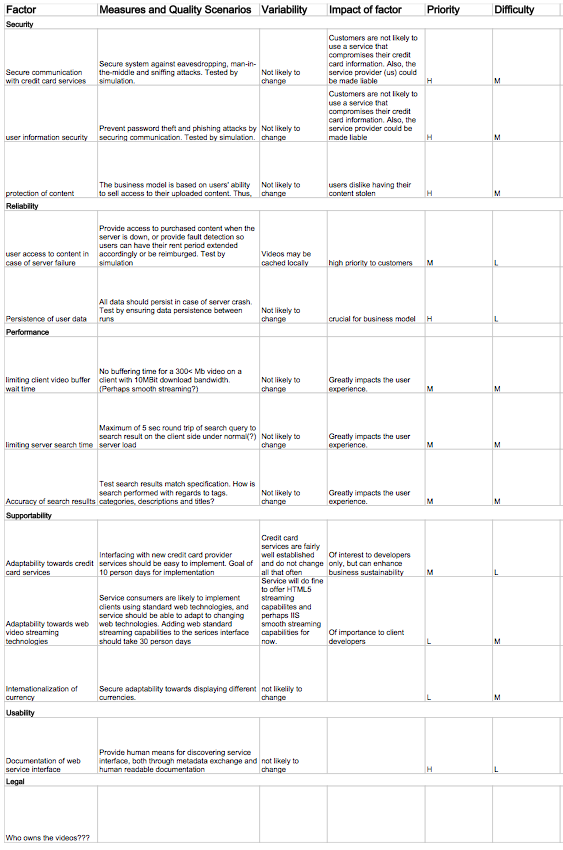
\includegraphics[scale=1.3]{FactorTable.png}
\end{center}
The factors are mainly defined by the business model, in that making changes to the business model, would change the non functional requirements of the system.  For example, the decision to include user generated content greatly impacts security of the system factors such as protection of video content in the system, as this in some sense is the property of the user who uploaded it.

Some of the usefulness of the factor table is its recording of quality scenarios, because it encouraged the group to reflect on quantifying the requirements, as to make them testable. Realistically, it would not be possible to satisfyingly implement and test all of the factors, but for the sake of exercise, the factor table was composed as if it was meant to be used in a real world situation. As a consequence of the limited timeframe of the project, most of these were not pursued.

\section{Data Modelling}
Another major part of our problem analysis was devising a model of the data, partly in order to construct and refine a database design for persisting the necessary data, and in part to serve for inspiration for C\# classes.
This modelling was done using  an ER-diagram as an aid for reflecting on a useful database design. This artefact serve as the basis for discussions in this section.

\subsection{ER-Diagram}
The ER diagram on the following page reflects our considerations on designing a useful relational database. The video and user entities constitute the bare minimum of required data to implement the core functionality of video streaming and user management, and the remaining entities capture the data needed to record either deposits and payments, or the data needed to perform statistical analysis for e.g making recommendations to individual users.
\begin{center}
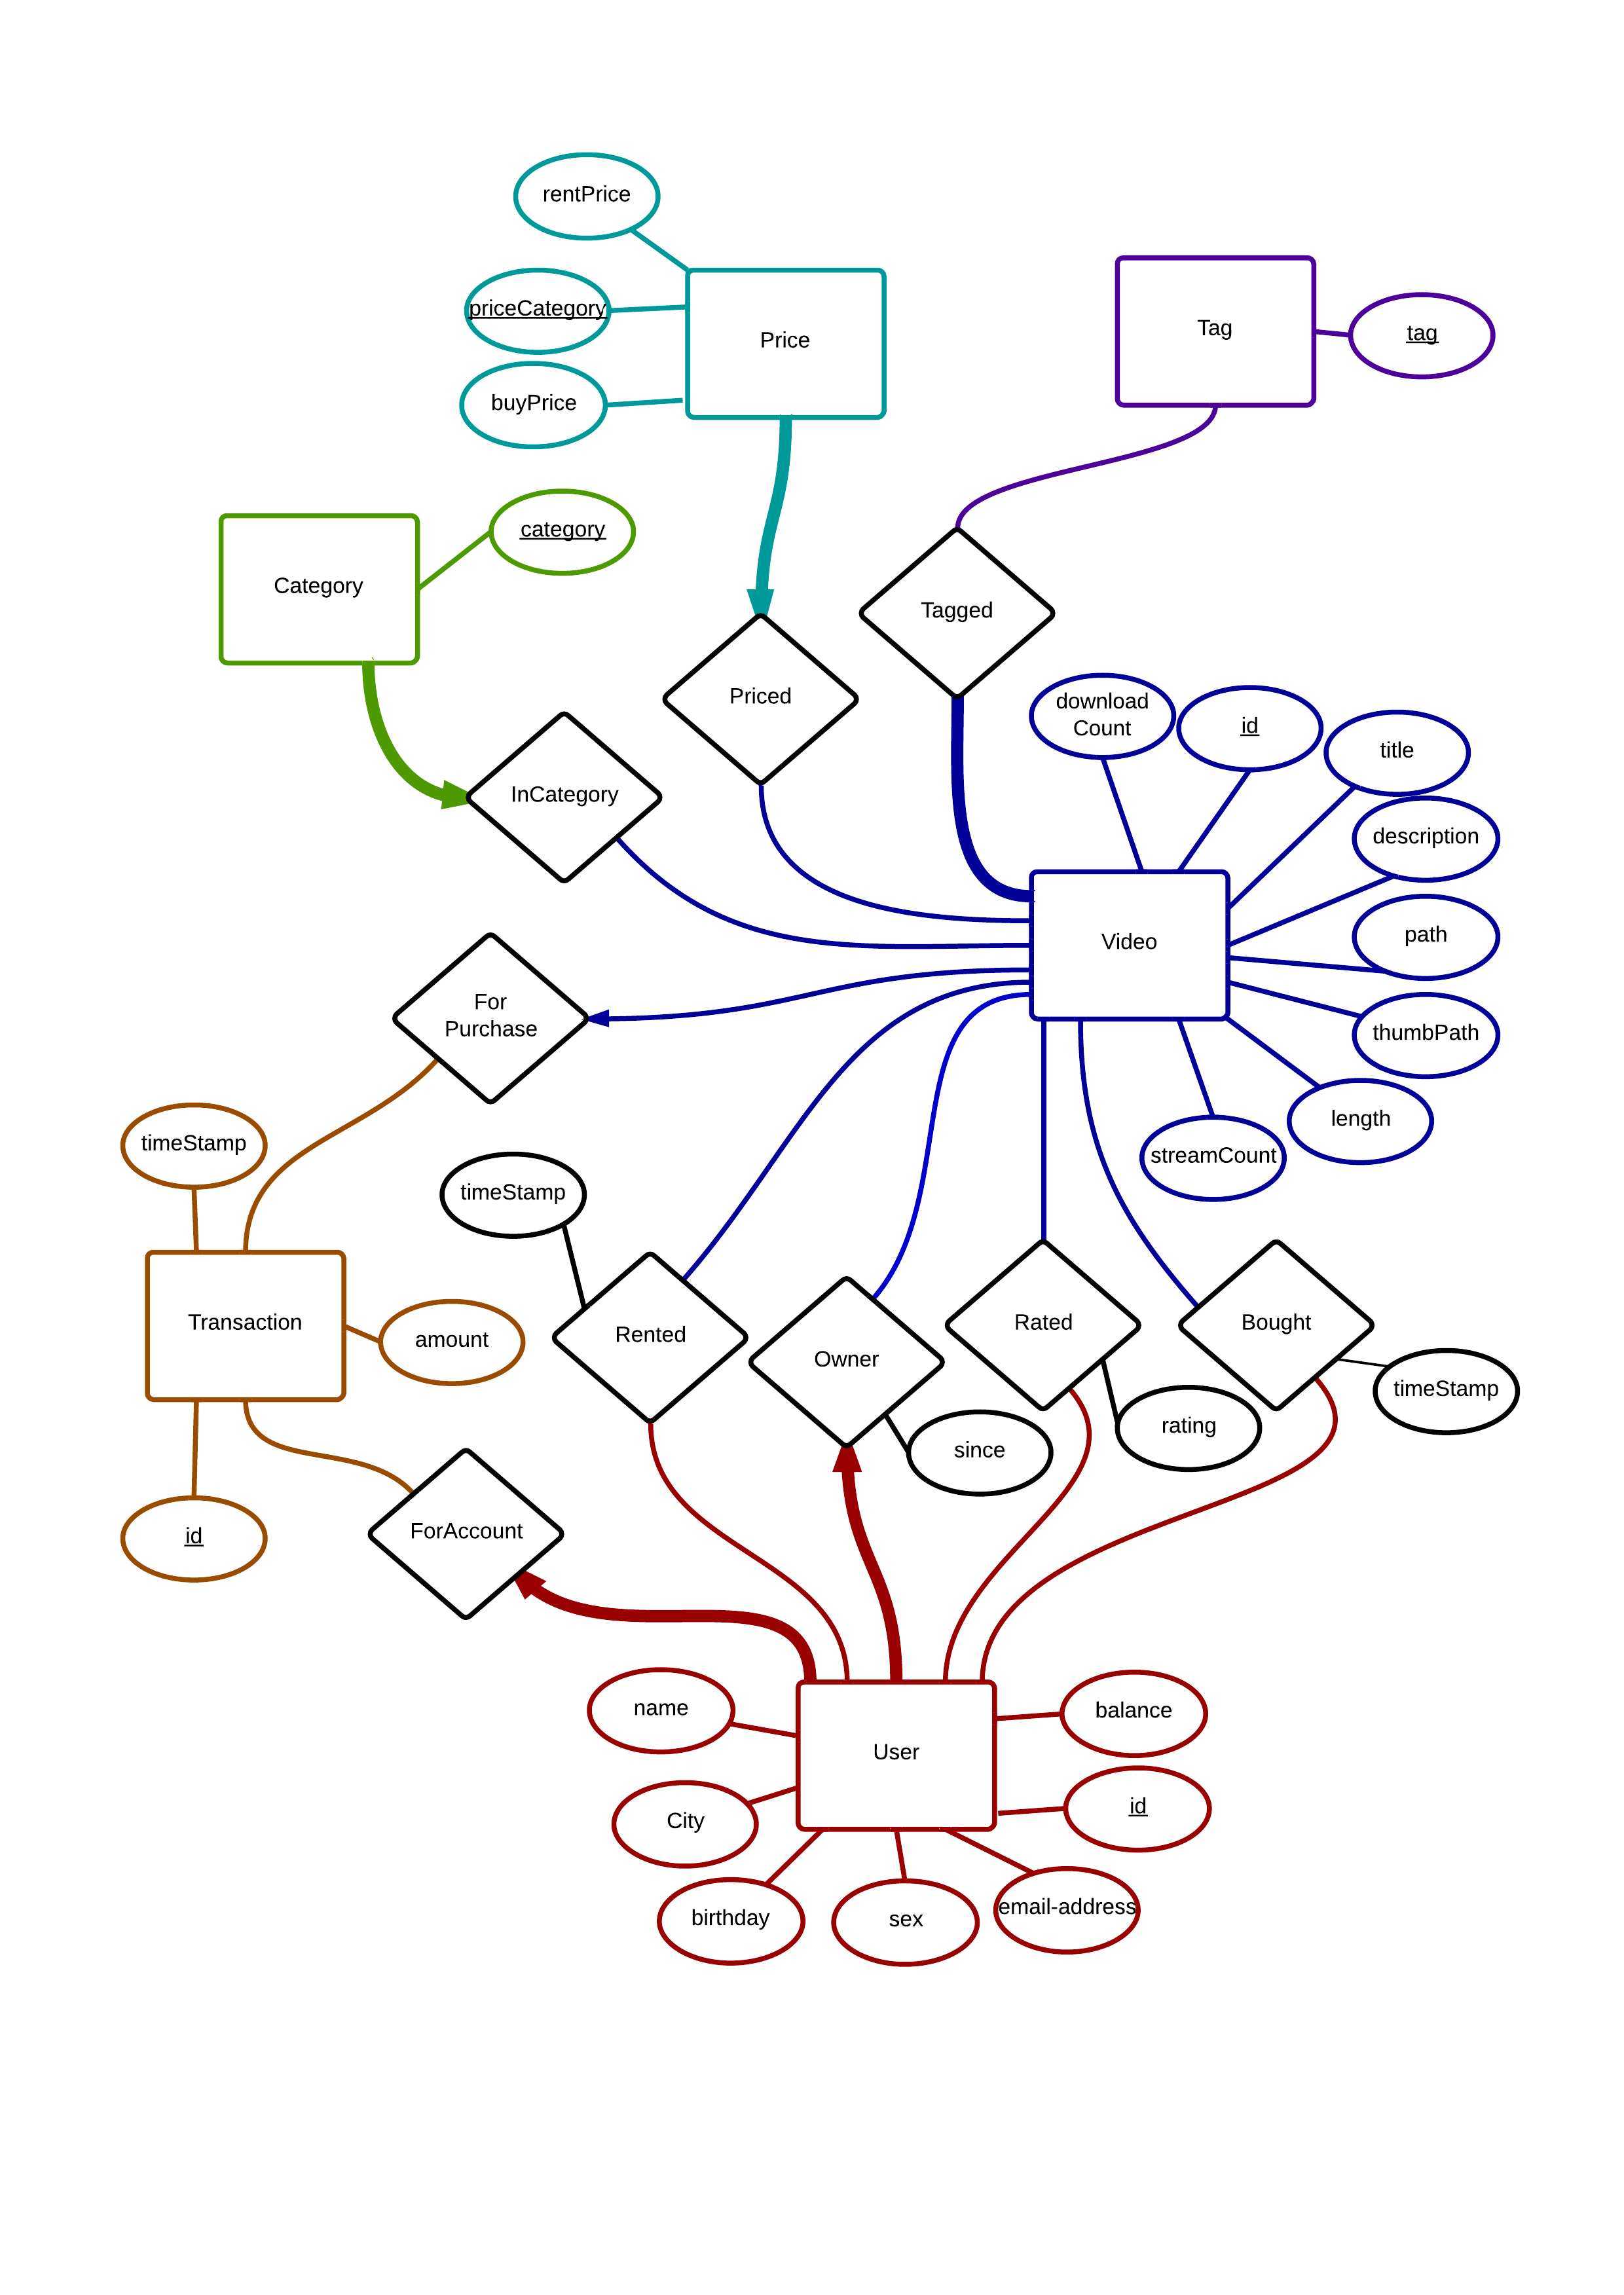
\includegraphics[scale=0.15]{ERDiagram.png}
\end{center}

The "transaction", "rented", and "bought" tables combined, capture the financial activities of the users, in that transactions capture deposits, or payments by users for videos, and the "rented" and "bought" tables capture the respective purchase histories of users.
We later realised that this design is flawed, as it allows for inconsistency between recorded purchases and financial transactions. A better design would have been to record a transaction with each rent or buy history, and discard recording videos associated with a financial transaction directly in the transaction table.

Another noteworthy detail is the relationship between the price table and the video table. The reason to keep prices enumerated by category in a separate table, as opposed to recording it directly in the video table, is the business model requirement of allowing user generated content. Defining a set of price categories that uploaders could choose from, simplifies the upload process as well as maintaining consistent pricing for different videos.

The shoppingcart entity was added to accommodate a wish from the SMU group of working with shopping cart functionality. Originally, the intent was for users to simply pay directly for each video separately when viewing it, either by renting or buying it. However, it was implemented since the requirement for shoppingCart functionality was negotiated by the SMU group and ourselves. Because of the design of the model, it was fairly easily added.

\section{Architectural Analysis}
In this section we will outline our efforts towards translating the functional and non-functional requirements into a large scale organization of system namespaces, that is to say, the logical architecture of the system. This is modelled using an UML package diagram, which will serve as the basis for the discussion. In addition, we will discuss available technologies and frameworks which are worth considering for meeting the requirements identified in the analysis.

\subsection{Package Diagram}
The package diagram below reflects the responsibilities identified by developing the use cases, and in part the non-functional requirements of the factor table. For example, the need for restricting access to videos dictates the existence of modules handling authentication and authorization, which in the model is delegated to the UserManagement package. The level of abstraction used in the diagram is very high, and is intended as inspiration for classes and namespaces and for improving the understanding of the system, but not as an exact specification.
\begin{center}
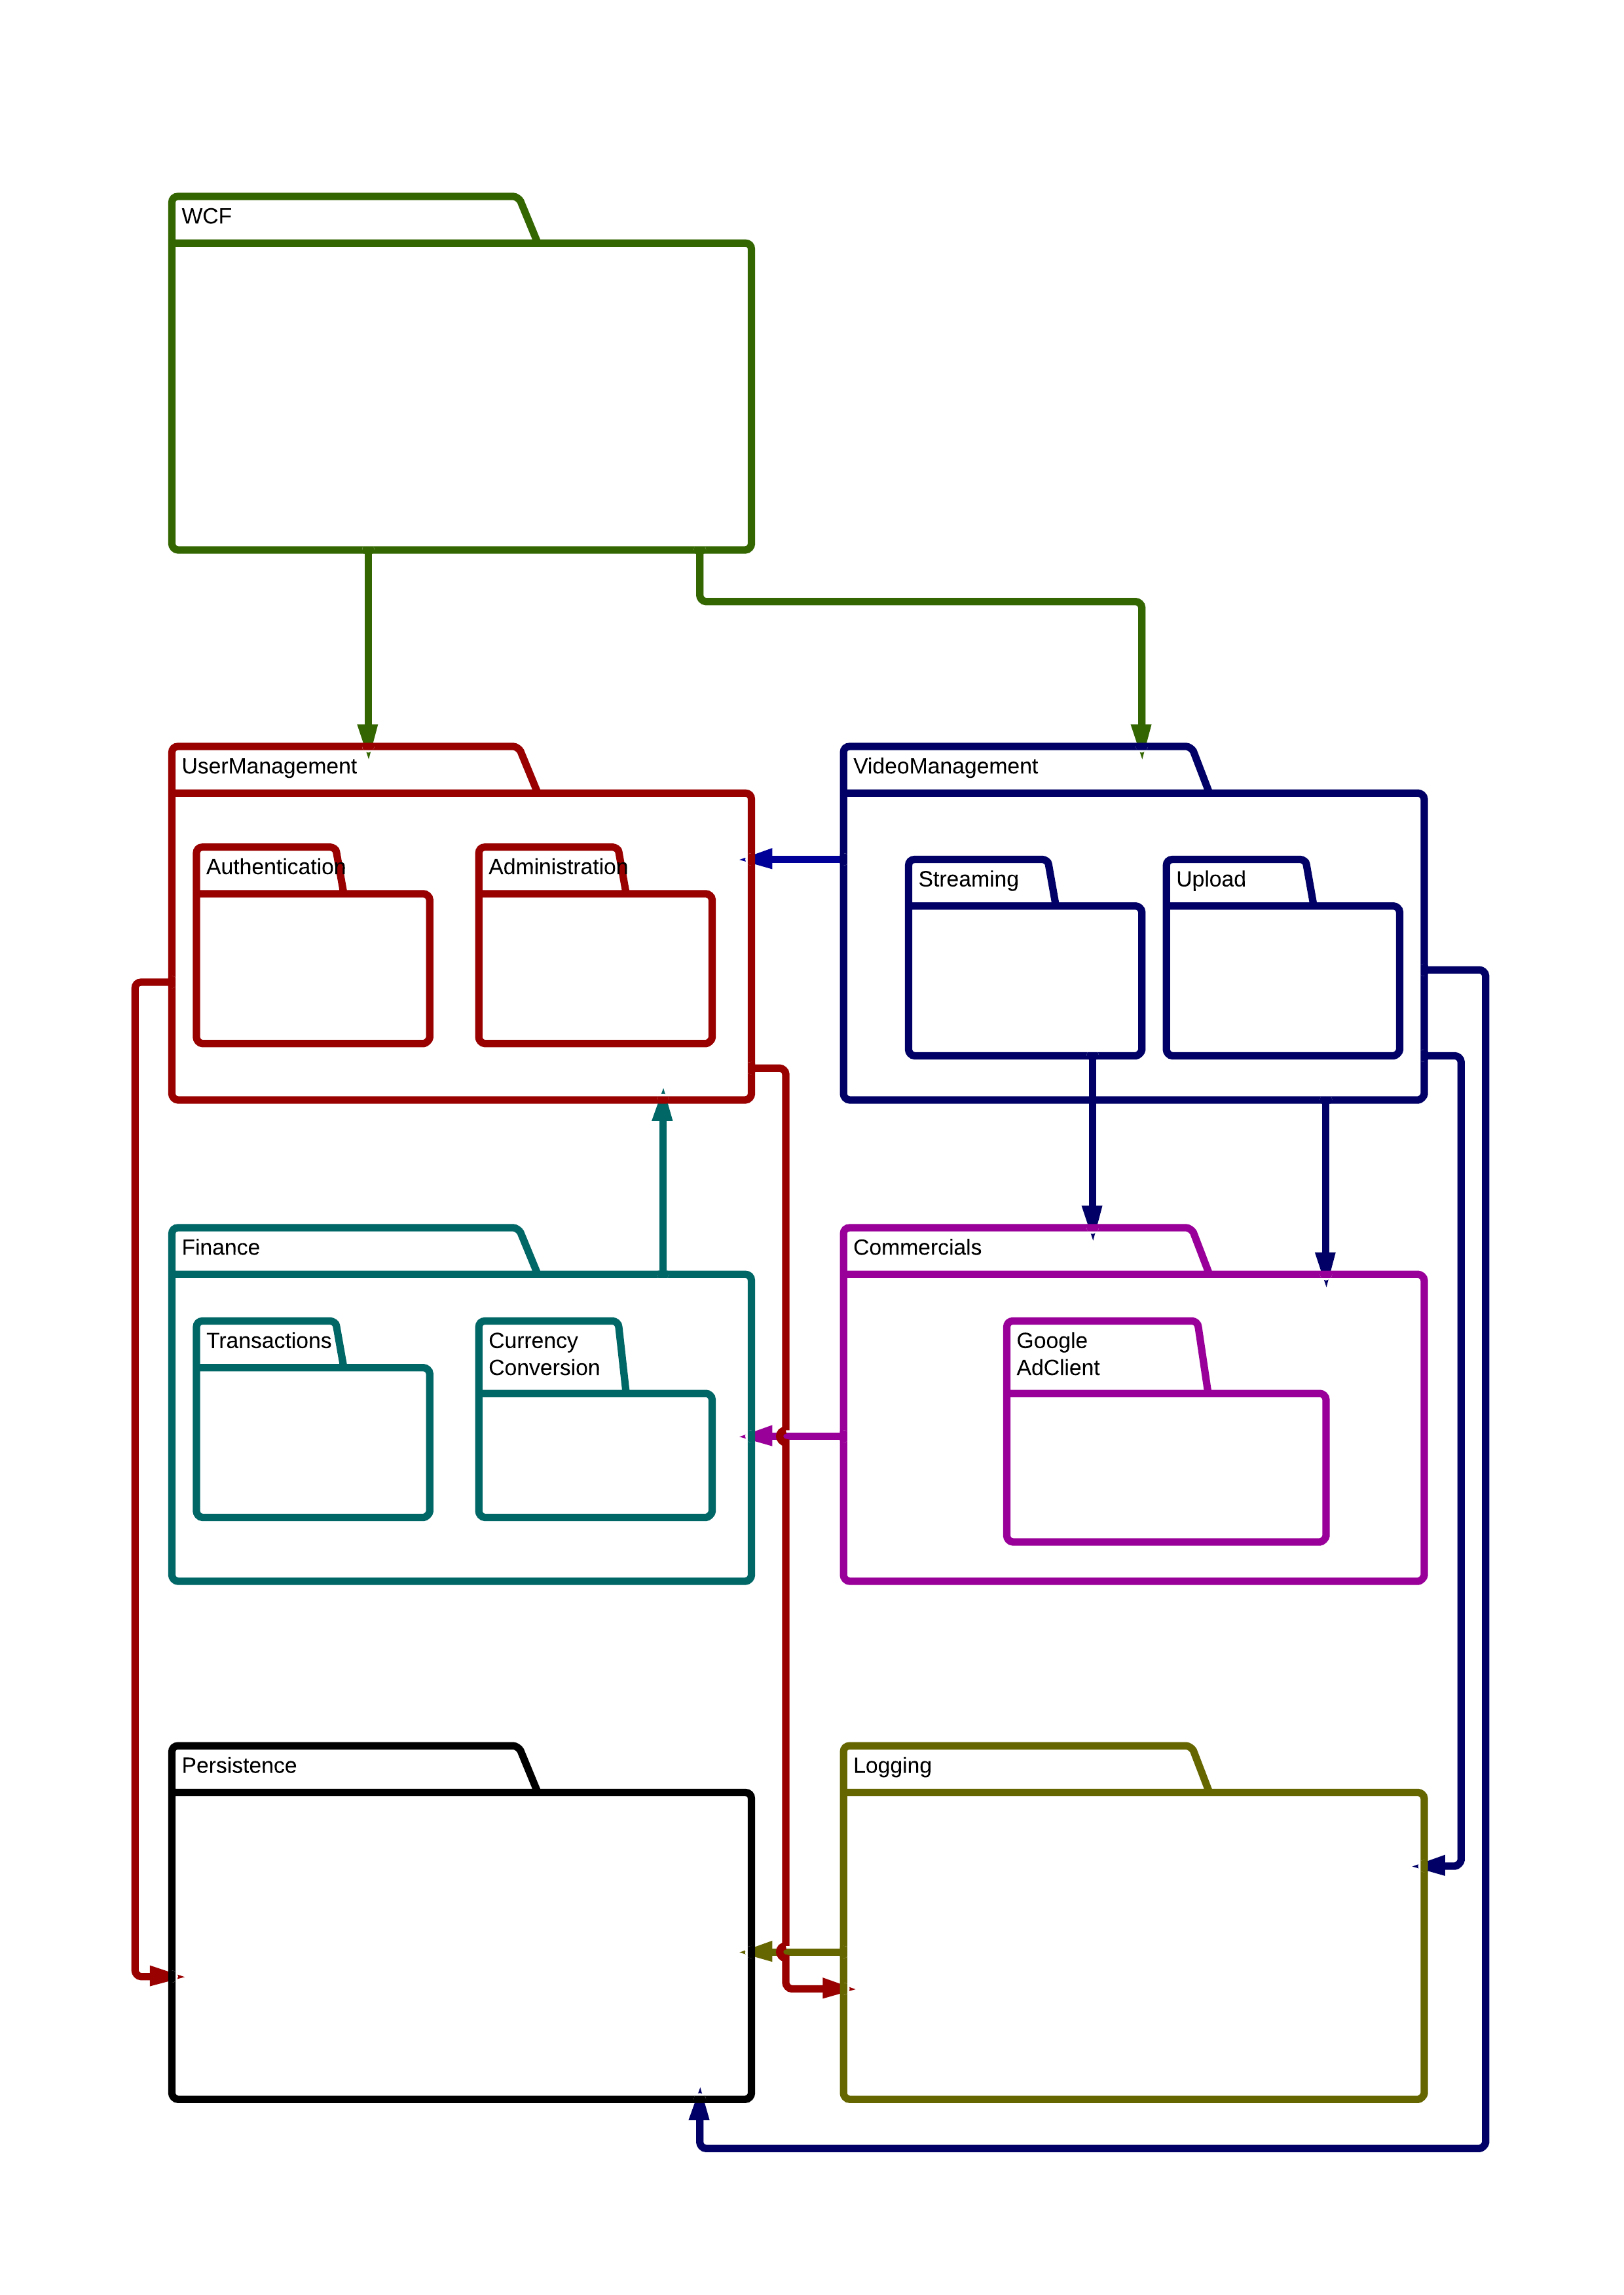
\includegraphics[scale=0.15]{PackageDiagram.png}
\end{center}

The WCF package assumes the responsibility of exposing the service interface to clients, including which ever configuration is necessary for achieving this. Responsibility of adding items to, removing items from, emptying, and checking out the shopping cart is delegated to the Finance package, in addition to making deposits to the users' RentIt credit balances.
The VideoManagement package is responsible for creating streams for the appropiate video files upon request, as well as generating links that can be used to download videos, in addition to limiting access to these links, as to make them available only to paying customers. Finally, the Persistence package is responsible for saving data and coordinating requests to the underlying persistence technology.

A detailed discussion of possible technical approaches to realising the requirements within the proposed architecture is deferred to the next section.


\subsection{Technology Considerations}
One of the goals of conducting a thorough analysis of the requirements and architecture of the system under development, is to make an informed decision on how to best use existing technologies and frameworks. In this section we will give the reader an overview of our thoughts on this subject. The following sections are structured by the topics they address:
\begin{itemize}
\item Web Service standard
\item Client video streaming
\item Security
\item Finance
\item Persistence
\end{itemize}

\subsubsection{Web Service Standard}
A formal requirement for the project is that the server is implemented using the Microsoft WCF framework. Consequential, the server operations will be exposed to clients using some web service standard. The WCF framework offers a wide variety of possible standards to let clients communicate with it. The major decision in the face of these possibilities, is choosing which message format is most appropriate; SOAP or REST.

Choosing the SOAP standard has the advantage of being the default WCF message format, which means using this option is likely to result in less configuration of the framework, thus saving the group some time and possibly hassle. In addition, SOAP works equally well over a multitude of different networking protocols, since it does not depend on the HTTP vocabulary, in contrast to REST, which provides some flexibility. This adds little value to the project however, as there is no good reason to use anything other than the HTTP protocol for communicating with clients.

Disadvantages of choosing SOAP over REST include the verbosity of the XML notation of SOAP messages, which cause them to be larger than the basic HTTP messages of REST. Moreover, the choice of service standard affects the ease with which different clients will communicate with the service. For example, choosing REST which returns and accepts JSON datatypes and therefore readily communicates with AJAX based clients, would make using  HTML5 video streaming quite easy. Using SOAP on the other hand would require a few extra contortions to extract the video information from the SOAP envelope, and play it using the HTML5 video element. On the other hand, .NET and Visual Studio have tools for working with the WSDL (Web Services Description Language) of SOAP services, in order to automatically serialize and de-serialize C\# data to SOAP envelopes. For this reason, streaming video clients written in C\#, such as WPF or Silverlight, should be straightforward to implement, when coding against a SOAP server.

Since the SMU group expressed preference to writing an ASP/AJAX client, there were strong arguments for supplying a REST service in order to make their lives easier. For implementing our own client, our group was partial to HTML5 video aswell (for reasons which will be discussed in the next section), which meant that REST seemed like the better choice. In the end, using the REST standard to implement the service was chosen because of its compatibility with HTML/AJAX.

\subsubsection{Client Video Streaming}
Another formal requirement for the project, was to implement a client for the RentIt service of our own. Firstly, this begs the question of whether to offer a desktop or web client. Offering a web client would allow it to be used on any platform that supports the web standards, which includes tablet and mobile devices. These devices could be supported by using a framework for adapting the user interface for the screen size of the specific device, like for example Bootstrap. Implementing desktop clients however, is much more familiar to the group, and could possibly save us some time for working on other features for the system. Most importantly, the group deemed the learning outcome of working with web technologies to be the greater of the two. Web technologies arguably play an increasing larger role in the landscape of IT products, and as such, familiarising ourselves with state of the art web standards would be well worth the effort. For this reason, the group chose to implement a web client rather than a desktop version.

After deciding on a web solution for the client part of the project, it was necessary to select the most appropriate technology for streaming video. The three major video streaming technologies, which can be considered web standards, are Flash, HTML5, and Silverlight.
Flash video streaming was off the table from the start, because it does not posses the quality of being a state of the art web standard, since it arguably has largely played out its role on the web. Working with Flash was not educationally interesting.

HTML, being the de facto standard of everything on the web, will probably always be relevant to be familiar with as a software developer. The multimedia capabilities of HTML5, are increasingly being used by product providers, and is supported by all browsers on all platforms. However, using HTML5 for streaming video would make it difficult to prevent users from downloading the videos to their own machines, for viewing even when the rent period had been exceeded. This is due the fact that HTML5 video treats the video elements like any other resource, such as for example a picture. This means that saving a video would only require the user to right-click the video element and select save as. Moreover, using HTML5 would make it cumbersome to use SOAP to communicate with the RentIt service, as discussed above, since the streamed data would have to be extracted from the SOAP envelopes and placed somewhere and in a format the HTML element could point at.

The third possible technology, Silverlight, suffers from some of the same diseases as Flash, in that Microsoft has abandoned the technology. There are a few commercial products that still depend on Silverlight, such as Netflix, but technologies that are not maintained by their providers are bound to disappear. As such the educational outcome of using is Silverlight is negligible. The technology does have the advantage however, of being part of the Microsoft technology stack, even though it is now considered legacy. This means that writing parts of the client in Silverlight could take advantage of the tools for working with SOAP services with WSDLs, which is the default service standard for WCF, meaning that the team could be spared of writing lines of boilerplate code.

The HTML5 solution was chosen as the technology for handing video streaming for the following reasons:
\begin{itemize}
\item More interesting from an educational point of view
\item More broadly supported by browsers and mobile platforms
\end{itemize}

\subsubsection{Security} \label{Security}
The business model depends on the system being secure in a number of different regards. Firstly, the system must provide some means of offering authentication and authorization of users, in order to make sure that users will only be granted access to content once they have paid for it, and in the appropriate time frame. In addition, it should not be possible for a user to download a video, unless she has permanently bought it.

WCF in itself provides tools for handling authentication and authorization, based on the ASP.NET authentication framework!!REFERENCE TIL LEARNING WCF KAPITEL 7. Using that, it would be possible to implement a fairly generic login architecture. However, in the past few years, a different approach to authenticating users have become quite popular; namely using web identity providers. By this approach, users log in with an account registered with a well known and widely used third party service, such as Facebook, Google or Windows Live. This is convenient for users since they then need to remember less usernames and passwords. From an educational perspective, it would also be interesting because it would allow the project group to get hands on experience with service oriented architecture, since these identity providers work by providing a service API. In addition, the default WCF identity mechanisms require credentials to be formatted in a specific manner, and placed in the authorization header of the HTTP message. Using e.g Facebook authentication, involves passing around a unique string, which can be used to access a users' information!!REFERENCE TIL FACEBOOK DOKUMENTATION. This gives us a little more freedom for making simplifications to the login architecture. For those reasons we decided to focus on using identity providers, rather than using the default WCF authentication framework.

As mentioned, preventing users from using the streamed data obtained by renting a video to download a video to their own hard-drive is also an important security issue. This is a difficult problem to solve since when a user is streaming the video data in their browser, regardless of which technology is used, they already have access to the data. This is exemplified by the myriad of rippers that exist for other media solutions such as Youtube, Spotify, Soundcloud or Netflix to name a few. For this reason, it seems unlikely that we would solve this problem in this project, since our focus was with managing a project with a geographically dispersed team, and not finding technical solutions to preventing content theft. As such, although we are aware of the issue, we have deemed it outside of the scope of this project.

Since sensitive information is passed by the client to the service, such as login and credit card information, implementing a secure communication channel between two is an important security issue as well. An obvious approach to this would be to use SSL encryption to establish a HTTPS connection, since this can all be handled automatically by the WCF framework and the IIS hosting environment!!REFERENCE TIL LEARNING WCF KAPITEL 7 OG MSDN. However, configuring the server on which  the IIS environment is running requires rights that are not granted to students, so this would have to be done by the course lecturer, in addition to all subsequent changes to the certificate. For this reason, we have decided to delimit the project to not include encryption.

\subsubsection{Finance} \label{Paypal}
Users pay for videos using a credit card. This means that the credit card needs to be validated by some external system, in order to ensure that the card is valid. Again we have decided to take advantage of service oriented architecture, by using PayPal as a merchant service provider. PayPal has a sandboxed service endpoint which makes testing easy, without using an actual credit card.

\subsubsection{Persistence}
Microsoft SQL Server is installed on the server, which is the most obvious choice for persisting data. However, it might be worth considering using a Object Relational Mapping framework to translate from C\# objects to relational tables, in order to save writing a substantial number of lines of boilerplate code. The ORM framework included in .NET is called Entity Framework, which is fairly well integrated with Visual Studio: tools include GUI editing of table mappings, discovering so called EntityObjects through connecting to a database, just to name a few. In addition, the Entity Framework works very well with the .NET LINQ construct, in that it is possible to query the so called EntitySets with LINQ queries, which is then translated to SQL.

Another possibility is a framework called NHibernate, which offers much of the same functionality, but is not as tightly integrated with Visual Studio. Because of our familiarity with the Entity Framework, we decided to put it to use, in order to reduce development time on the persistence module of the system.

\section{Project Management Plan}
To manage the development phase of our project, we have utilized different methods and tools, trying to optimize our work flow and organizing the work that needed to be done. \

We have applied the SCRUM method during our implementations. As an agile development technique, we have chosen this, to try and be more flexible in our work, especially considering our international collaboration. As we expected, some adjustments to our requirement had to be made in accordance with the SMU team, and to some degree SCRUM help handle these. But there were times when the opposite were true, and the changes to our work were too great. A more in-depth look at our work with agile methods and dispersed collaborations can be read in the SMU Collaboration section on page \pageref{SMU Collaboration}.
